\documentclass[10pt,twocolumn]{article}

\usepackage[margin=0.72in]{geometry}
\usepackage{graphicx}
\usepackage{booktabs}
\usepackage{array}
\usepackage{amsmath}
\usepackage{amssymb}
\usepackage{hyperref}
\usepackage{xcolor}
\usepackage{caption}
\usepackage{subcaption}
\usepackage{enumitem}
\usepackage{float}
\usepackage[section]{placeins}
\usepackage{balance}

\graphicspath{{../figures/}}

\definecolor{bggorange}{HTML}{FF8A2A}
\definecolor{bggdark}{HTML}{1D2A35}
\definecolor{bggblue}{HTML}{3F3A60}

\hypersetup{
    colorlinks=true,
    linkcolor=bggblue,
    citecolor=bggblue,
    urlcolor=bggblue
}

\setlength{\columnsep}{0.24in}
\setlist[itemize]{leftmargin=*, topsep=2pt, itemsep=1pt}
\setlist[enumerate]{leftmargin=*, topsep=2pt, itemsep=1pt}

\title{\vspace{-0.6cm}\textbf{Beyond Communities and the Shared Canon Layer in BoardGameGeek Co-Ownership Networks}}
\author{Ahmet Ihsan G\"ul\\
\small CS514 Network Science, Sabanc\i{} University}
\date{}

\begin{document}

\twocolumn[
\begin{@twocolumnfalse}
\maketitle
\begin{abstract}
BoardGameGeek (BGG) catalogs board game collecting through user-curated ownership records, providing a hobby-wide behavioral signal that remains underanalyzed at the network level. This project analyzes a bipartite ownership matrix of 5,504 active collectors and 2,500 ranked games through a dual-method pipeline that combines network science and matrix decomposition. On the graph side, a Newman user-normalized projection was filtered with the Serrano-Boguna-Vespignani disparity backbone filter ($\alpha=0.025$) and clustered with Louvain modularity ($\gamma=1.75$). On the matrix side, Non-negative Matrix Factorization (NMF) was applied directly to the raw ownership matrix to test whether the same latent taste structures emerge without projection. Parameters were selected through joint stability-significance screening, yielding median pairwise NMI $=0.758$ and a modularity $z$-score of $27.31$ against a degree-preserving null model. The graph and matrix methods independently recovered 8 of 11 taste dimensions with median cosine similarity $0.674$, showing that the two approaches reinforce one another. The 43 detected communities decompose into nine behavioral types, including taste specialists, cross-over groups, temporal canon communities, temporal artifacts, bridge clusters, bridge singletons, shared-culture groups, franchise series, and small fragments. User profiling across 11 named taste dimensions plus a residual category shows that 62.9\% of eligible collectors are organized primarily by a shared-canon layer rather than by a single taste identity. Together, these findings reveal a two-layer hobby structure made of differentiated taste identities and a shared canon layer that cuts across them.
\end{abstract}
\vspace{0.2cm}
\end{@twocolumnfalse}
]

\section{Introduction}

BoardGameGeek is the dominant online database for modern board gaming. Its records include game metadata, ratings, rankings, comments, plays, and user-maintained collections. Most BGG analyses emphasize ratings, ranks, game weight, or curated metadata such as mechanics and categories. This project instead focuses on ownership, meaning what users choose to keep in their collections.

Ownership is useful because it is a behavioral signal. A rating expresses an opinion about one game, while an owned collection expresses a relationship among many games. If many users own two games together, that pair may share audience, genre, era, market position, franchise logic, or cultural role. The central question is therefore the following.

\begin{quote}
\emph{What does co-ownership reveal about how the board game hobby is organized, and what does it expose at the boundaries of official metadata categories?}
\end{quote}

The final interpretation is two-layered. BGG ownership contains recognizable taste communities, but it also contains a shared-canon layer made of recent releases, broad-appeal bridge games, and franchise systems that cut across narrow genre identities.

\section{Data Collection}

\subsection{BGG API and Metadata Sources}

Data were collected from BoardGameGeek during April 2026, with the baseline reliable-user snapshot recorded on 18 April 2026 and the diversity-expansion snapshot recorded on 23 April 2026. BGG ranks and ownership states should therefore be interpreted as a time-specific snapshot rather than as permanent attributes.

The project used BGG's public XML API2 and related BGG data pages. The main API base was \url{https://boardgamegeek.com/xmlapi2}. Game records and metadata were collected from BGG rank and game-detail sources, while user collection records were fetched with the collection endpoint. A practical implementation finding was that \texttt{collection?username=USER\&stats=1} returns collection status and user rating information in one call, making separate rated-only collection calls unnecessary for this project.

The game universe was fixed at 2,500 ranked games. Metadata such as mechanics, categories, year, rank, rating, and weight were stored as node attributes and used for interpretation only. Metadata was not used as input to community detection.

\subsection{User Discovery and Reliability Filtering}

The initial user pool was seeded from users interacting with top-ranked BGG games. Candidate usernames were discovered from game-level rating comments and play logs. These interactions provided candidate users, but the full collection structure was obtained only after fetching each user's BGG collection.

Reliable collectors were defined by an explicit rule. The collection fetch had to succeed, the user had to have at least 50 total collection items, and the user had to overlap with at least 10 games in the selected 2,500-game universe. The baseline sweep discovered 7,535 candidate users, fully fetched 6,519 users, and retained 5,175 reliable users.

\subsection{Diversity Expansion}

The baseline user pool was dense but biased toward high-visibility mainstream BGG users because it was discovered through the top-ranked game ecosystem. To reduce this sourcing bias, a second isolated sweep targeted mechanics and categories that were underrepresented in the baseline. Expansion seeds included taxonomy-deficit games, rank-stratified games, and wishlist-ratio contrast games.

Candidate users in the expansion were discovered by the same interaction-based strategy and then enriched with one \texttt{collection?stats=1} request per user. The strict expansion reliability rule again used at least 50 collection items and at least 10 selected-game overlaps. A looser community-only pool was also tracked internally using at least 20 collection items and at least 3 selected-game overlaps, but the main analysis used the strict reliable pool. The expansion produced 478 strict reliable users and improved 28 of 30 target underrepresented tags by at least 20\%. The merged final matrix contained 5,504 active collectors and 2,500 games.

\subsection{Reproducibility}

The analysis was implemented in Python. Processed data, notebooks, scripts, and report figures are organized in the submitted project repository. Key scripts include \texttt{cs514\_parameter\_sweep.py}, \texttt{cs514\_detect\_communities.py}, \texttt{cs514\_nmf\_test\_a.py}, \texttt{cs514\_nmf\_test\_b.py}, \texttt{cs514\_build\_user\_profiles.py}, and \texttt{cs514\_analyze\_user\_archetypes.py}.

\begin{table}[!htbp]
\centering
\caption{Final ownership dataset used for the main analysis.}
\label{tab:data}
\begin{tabular}{lr}
\toprule
Quantity & Value \\
\midrule
Reliable collectors/users & 5,504 \\
User-profile eligible users & 5,125 \\
Games & 2,500 \\
API requests & 26,911 \\
Ownership records & $\sim$437K \\
Matrix density & 3.4\% \\
\bottomrule
\end{tabular}
\end{table}

\begin{figure}[!htbp]
\centering
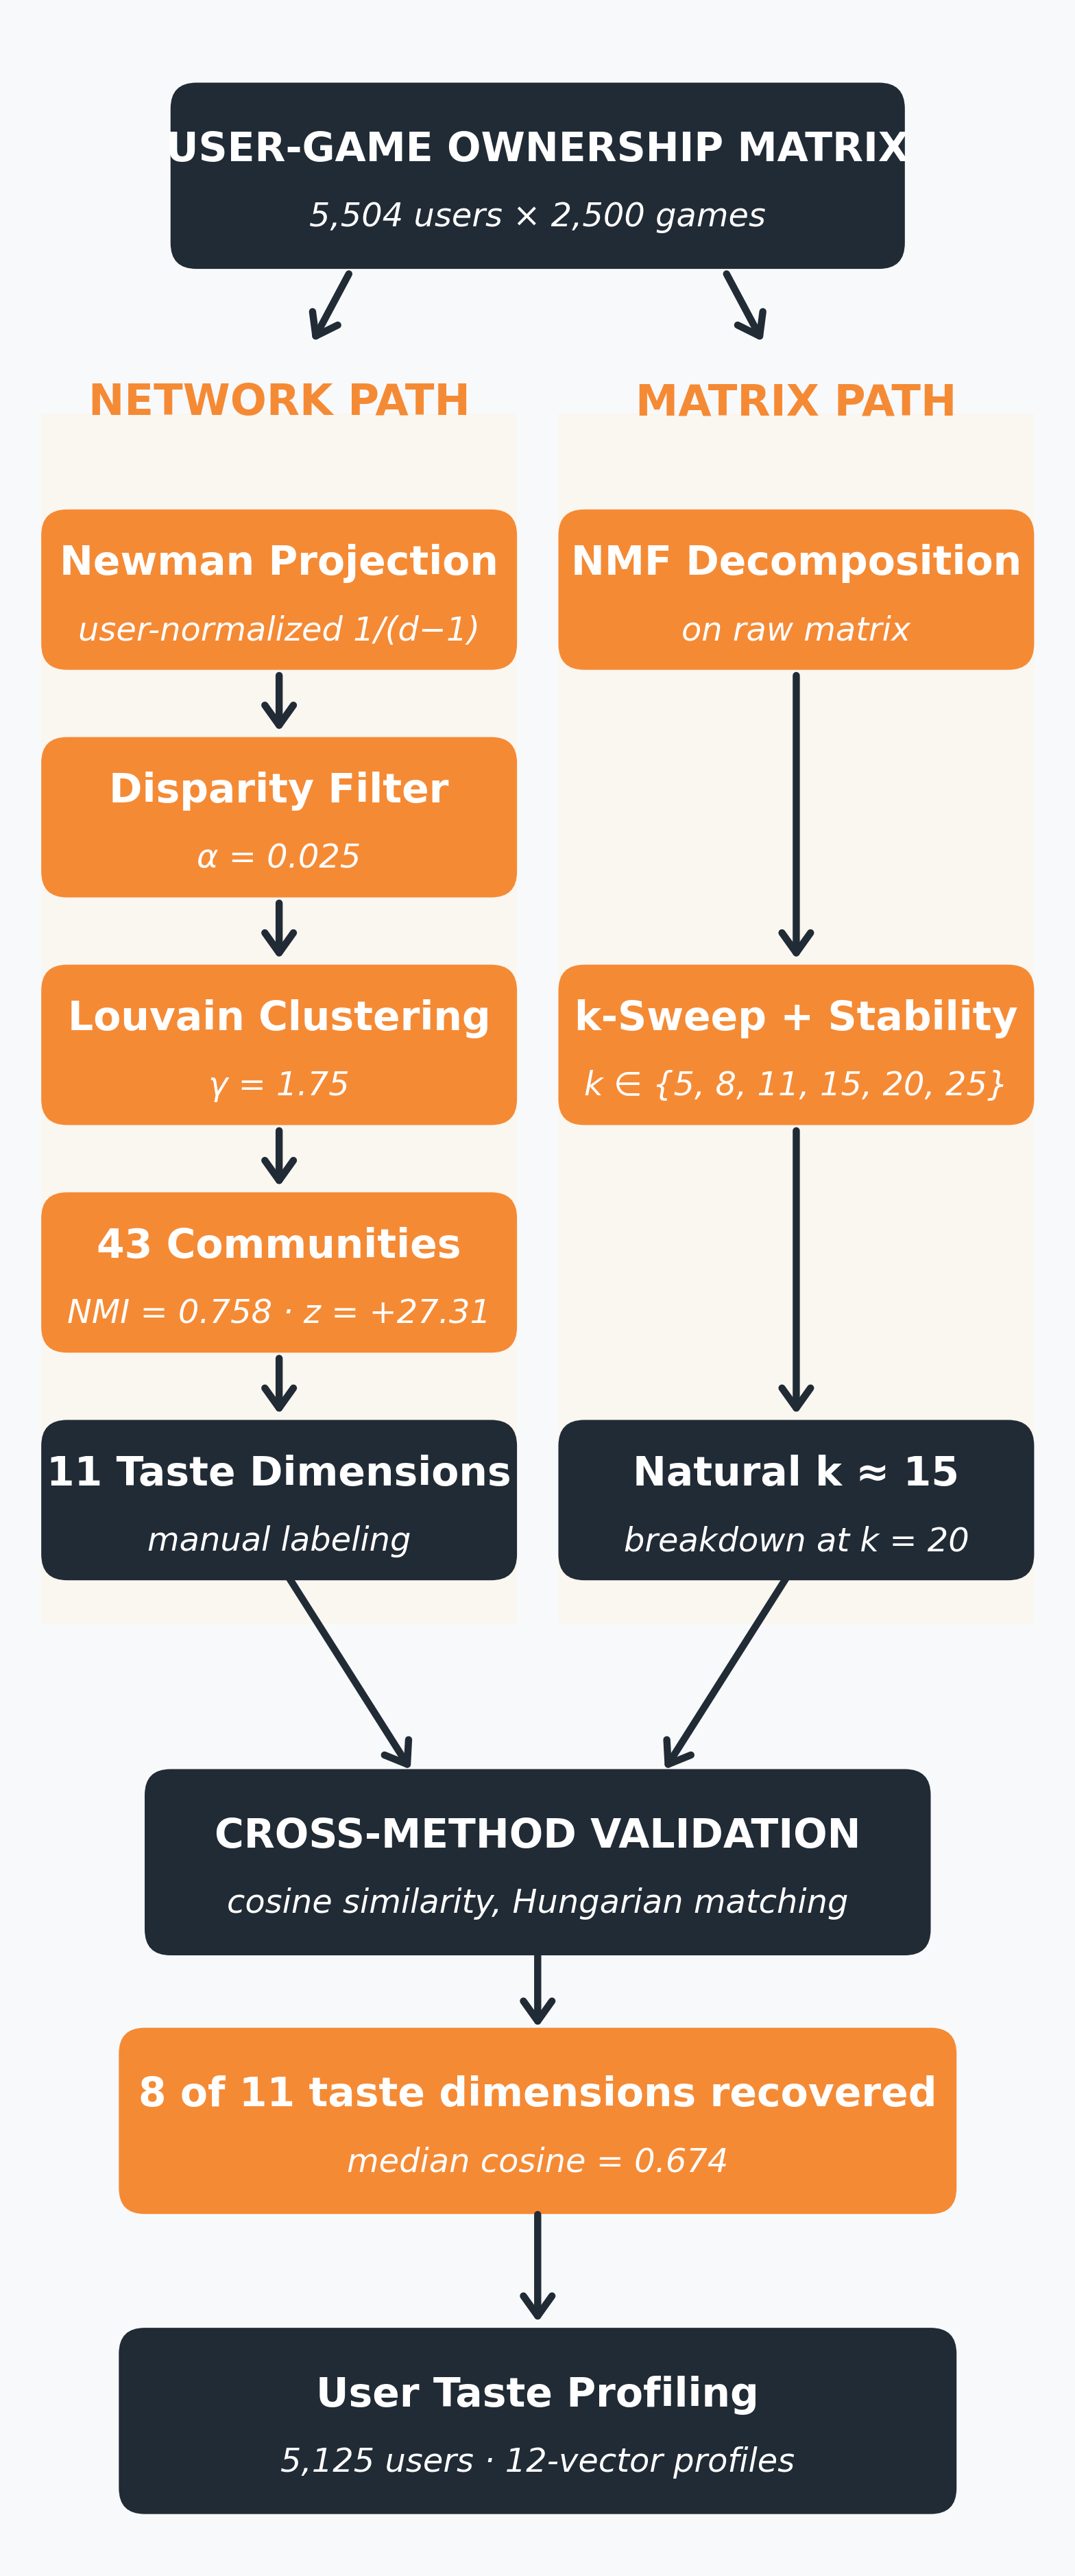
\includegraphics[width=\linewidth]{figure1_pipeline_diagram.png}
\caption{Overview of the dual-path analysis. The graph path extracts a statistically filtered co-ownership backbone and detects communities, while the matrix path applies NMF directly to the ownership matrix. The two paths meet in cross-method validation and user profiling.}
\label{fig:pipeline}
\end{figure}

Figure \ref{fig:pipeline} summarizes the full workflow from the ownership matrix to graph-side communities, matrix-side latent components, and user profiles.

\section{Graph Construction}

\subsection{Bipartite Ownership Matrix}

Let $B$ be the binary user-game ownership matrix, where $B_{ug}=1$ if user $u$ owns game $g$ and $B_{ug}=0$ otherwise. Only current ownership was used to construct the primary graph. Ratings, comments, plays, wishlist, previous ownership, and other non-ownership signals were collected or inspected during the project, but they were excluded from the final network construction so that the main edge definition remained behaviorally clear.

\subsection{Newman User-Normalized Projection}

The bipartite graph was projected into a weighted game-game network using a Newman-style collaboration projection \cite{newman2001}. A user with $d_u$ selected owned games contributes weight $1/(d_u-1)$ to each pair of games in that user's collection as follows.

\begin{equation}
w_{ij} = \sum_{u} \frac{B_{ui}B_{uj}}{d_u - 1},
\quad d_u = \sum_g B_{ug}.
\end{equation}

This normalization reduces heavy-collector dominance. A user with thousands of games creates many pairwise co-ownership links. The Newman projection spreads that user's contribution across the pairs induced by their collection rather than allowing raw pair counts to dominate.

\subsection{Disparity Backbone Filter}

The projected game-game network is too dense to interpret directly. To extract a statistically meaningful backbone, the Serrano-Boguna-Vespignani disparity filter was applied \cite{serrano2009}. For node $i$, let $s_i=\sum_j w_{ij}$ be its strength, $k_i$ its degree, and $p_{ij}=w_{ij}/s_i$ the normalized weight of edge $(i,j)$ around node $i$. The edge-level local significance can be written as follows.

\begin{equation}
\alpha^*_{ij} = 1 - (k_i-1)\int_0^{p_{ij}} (1-x)^{k_i-2}\,dx.
\end{equation}

An edge was retained if $\alpha^*_{ij}<\alpha$ from at least one endpoint. The final backbone used $\alpha=0.025$. This local filter compares an edge against the weight distribution around each endpoint rather than against one global threshold.

\begin{table}[!htbp]
\centering
\caption{Main backbone topology at $\alpha=0.025$.}
\label{tab:topology}
\begin{tabular}{lr}
\toprule
Statistic & Value \\
\midrule
Nodes & 2,500 \\
Possible game-game pairs & 3,123,750 \\
Backbone edges & 214,379 \\
Density & 0.0686 \\
Average degree & 171.5 \\
Median degree & 94.0 \\
Connected components & 1 \\
Largest component & 2,500 nodes \\
Average clustering & 0.783 \\
ER expected clustering & 0.0686 \\
Average shortest path & 1.93 \\
Diameter & 2 \\
\bottomrule
\end{tabular}
\end{table}

\section{Community Detection and Parameter Selection}

\subsection{Louvain Modularity and Software}

Communities were detected with Louvain modularity maximization \cite{blondel2008}. The implementation used NetworkX's \texttt{louvain\_communities} routine with weighted edges and explicit random seeds. Newman projection, the disparity filter, graph diagnostics, and output generation were implemented in custom Python code. The main Python stack included NetworkX 3.6.1, scikit-learn 1.8.0, SciPy 1.17.1, pandas 3.0.2, NumPy 2.4.4, and Matplotlib 3.10.9. Leiden \cite{traag2019} is a natural future robustness check because it guarantees better-connected communities than Louvain.

The weighted modularity objective with resolution $\gamma$ is

\begin{equation}
Q(\gamma)=\frac{1}{2m}\sum_{ij}
\left[
A_{ij} - \gamma\frac{k_i k_j}{2m}
\right]\delta(c_i,c_j).
\end{equation}

Here $A_{ij}$ is the weighted adjacency matrix, $k_i$ and $k_j$ are node strengths, $m$ is total edge weight, and $\delta(c_i,c_j)$ indicates whether nodes $i$ and $j$ share a community.

\subsection{Tuning Procedure}

Two parameters were tuned, the disparity threshold $\alpha$ and the Louvain resolution $\gamma$. The broad sweep tested $\alpha \in \{0.001,0.005,0.01,0.025,0.05\}$ and $\gamma \in \{0.5,0.75,1.0,1.25,1.5,2.0\}$ with 10 Louvain seeds per cell. Candidate settings were then examined with a targeted 20-seed refinement around $\alpha=0.025$. Null-model $z$-scores were computed from 20 degree-preserving randomized graphs per tested setting.

The selection used two gates.

\begin{itemize}
    \item The stability gate required median pairwise NMI across Louvain seeds to be at least 0.70.
    \item The null-model gate required observed modularity to exceed the degree-preserving null with $z>2$.
\end{itemize}

The selected setting, $\alpha=0.025$ and $\gamma=1.75$, produced 43 communities, median pairwise NMI $=0.758$, observed modularity $\approx0.077$, null mean modularity $\approx0.068$, and $z=27.31$. It was selected because it was the finest resolution that passed both gates. Although the null model used 20 randomized graphs rather than hundreds of replicates, the observed modularity was 27 standard deviations above the null mean, which makes the significance conclusion insensitive to small changes in the estimated null variance. The network-side sweep is shown in Figure \ref{fig:network_tuning}, and the matrix-side sweep is shown in Figure \ref{fig:nmf_tuning}.

\begin{figure}[!htbp]
\centering
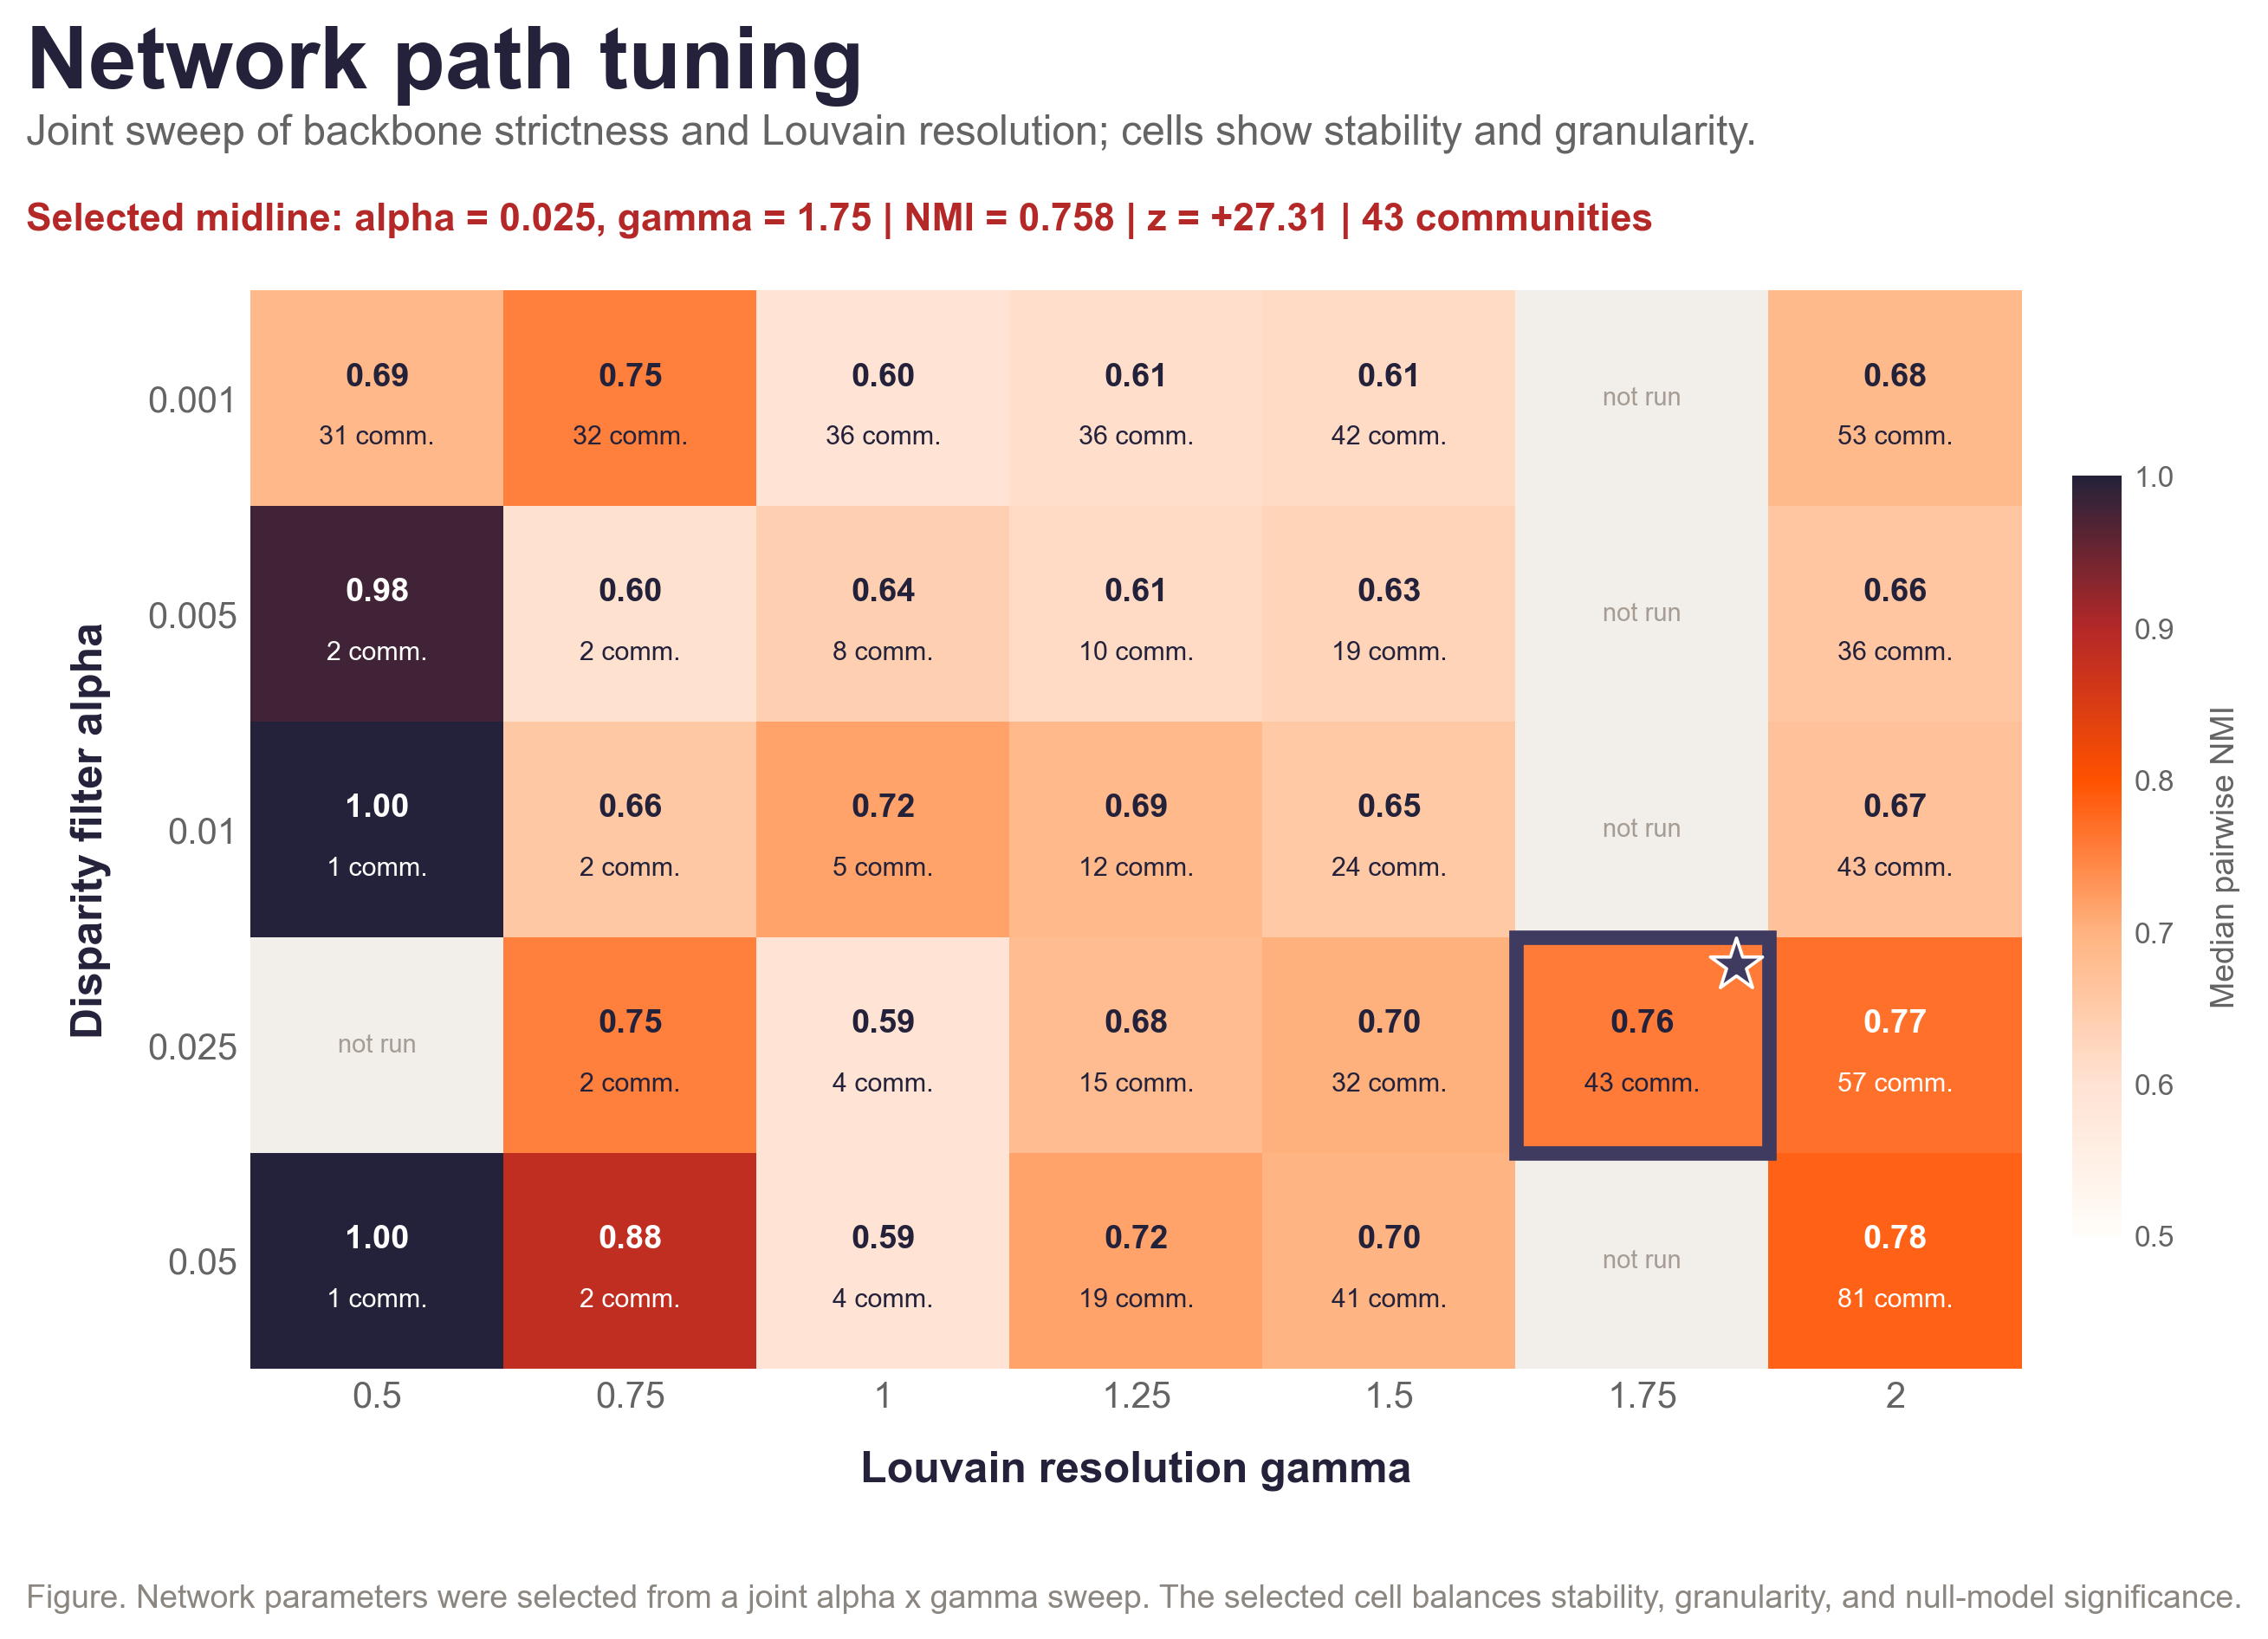
\includegraphics[width=\linewidth]{figure_methods_network_parameter_sweep_orange.png}
\caption{Network-path parameter sweep. The selected setting $\alpha=0.025$, $\gamma=1.75$ balanced stability, granularity, and null-model significance.}
\label{fig:network_tuning}
\end{figure}

\begin{figure}[!htbp]
\centering
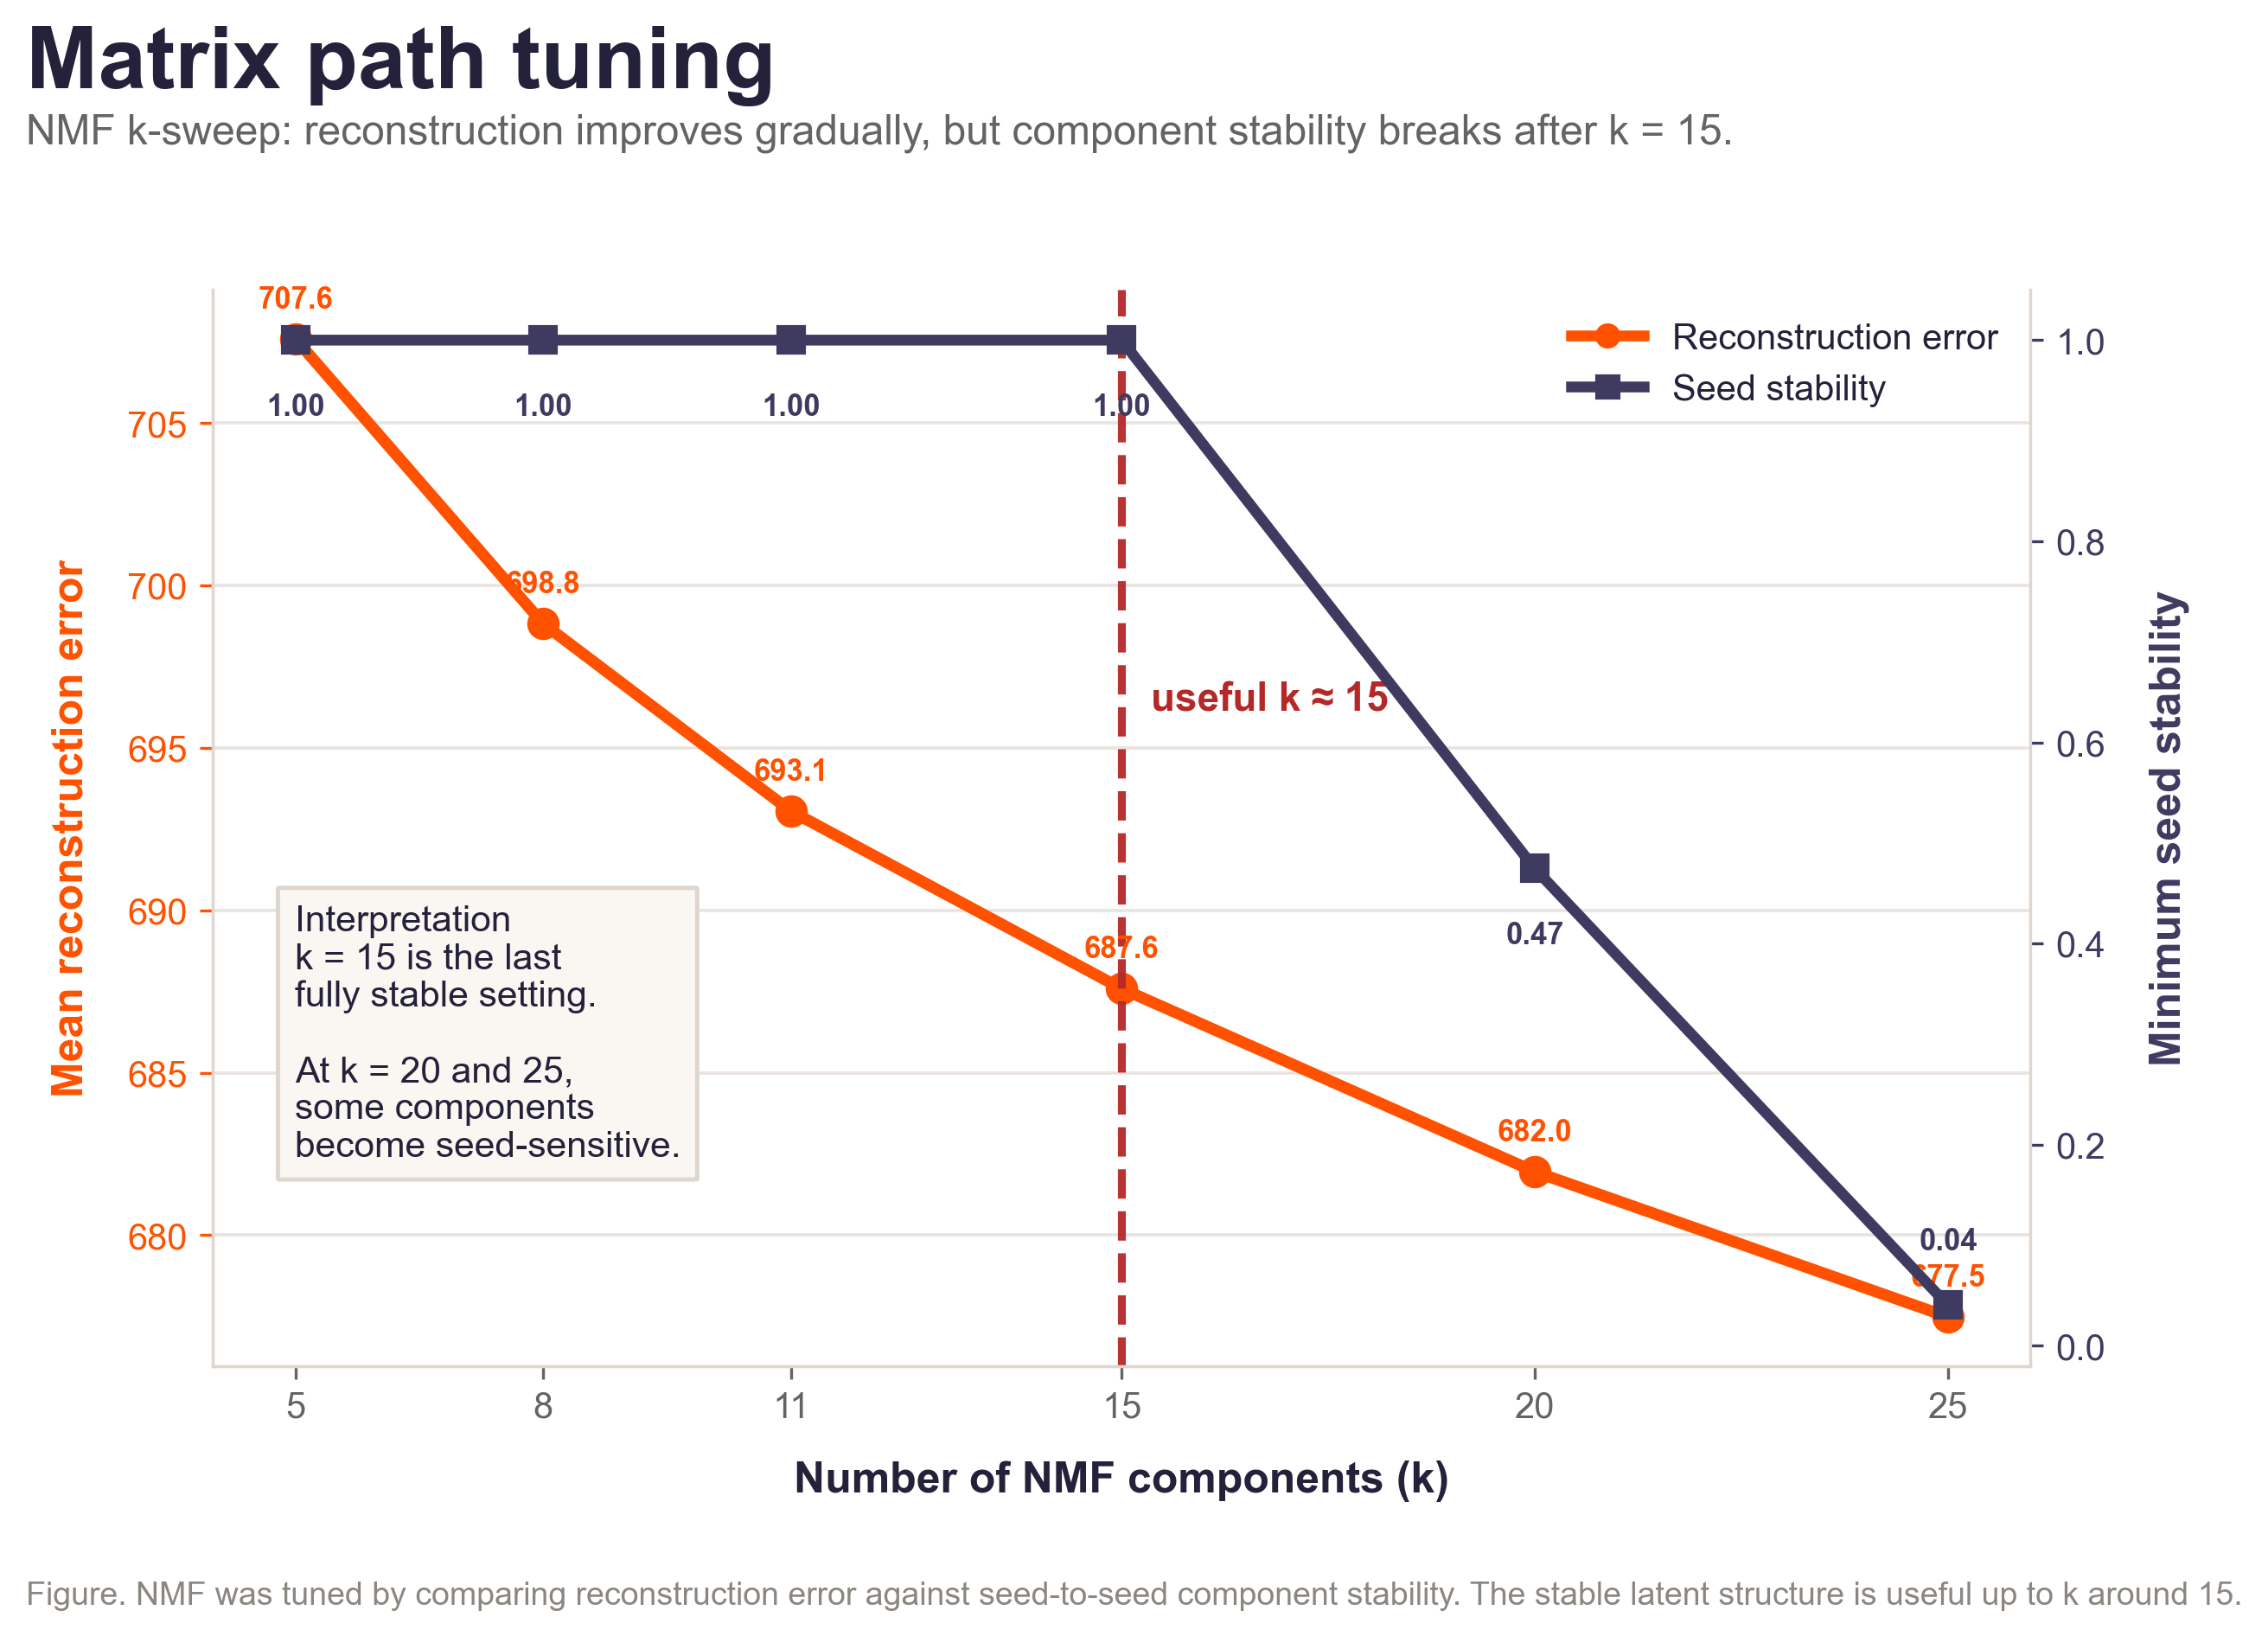
\includegraphics[width=\linewidth]{figure_methods_nmf_k_sweep_orange.png}
\caption{Matrix-path NMF sweep. Components remained stable up to about $k=15$, while larger decompositions became seed-sensitive.}
\label{fig:nmf_tuning}
\end{figure}

\begin{table}[!htbp]
\centering
\caption{Targeted 20-seed refinement and null-model validation at $\alpha=0.025$.}
\label{tab:tuning}
\begin{tabular}{rrrrrl}
\toprule
$\gamma$ & Comm. & NMI & $Q_{\mathrm{obs}}$ & $z$ & Decision \\
\midrule
1.25 & 15 & 0.680 & 0.124 & 135.18 & NMI below gate \\
1.50 & 32 & 0.703 & 0.094 & 69.22 & Valid, coarser \\
1.75 & 43 & 0.758 & 0.077 & 27.31 & Main setting \\
2.00 & 57 & 0.767 & 0.064 & -3.46 & Null fails \\
\bottomrule
\end{tabular}
\end{table}

The setting $\alpha=0.05$ retained 337,995 edges and had average degree 270.4, compared with 214,379 edges and average degree 171.5 at $\alpha=0.025$. Although $\alpha=0.05$ produced useful descriptive partitions, it admitted a denser backbone under a looser local significance threshold. The chosen $\alpha=0.025$ was therefore treated as a conservative midline, richer than the sparse $\alpha=0.001$ macro graph but less permissive than $\alpha=0.05$.

\section{Matrix Decomposition}

NMF was used as a second, projection-free view of the same ownership data \cite{lee2001}. NMF decomposes the non-negative ownership matrix $X$ into

\begin{equation}
X \approx WH,
\end{equation}

where $W$ gives user-component weights and $H$ gives component-game weights. Each row of $H$ can be interpreted as a latent ownership direction.

\subsection{Implementation and Test Design}

Implementation used scikit-learn's \texttt{NMF} with coordinate descent, Frobenius loss, tolerance $10^{-4}$, and sparse matrix input. Test A restricted the matrix to the games assigned to the 11 Louvain-derived taste dimensions, producing a 5,482 user by 1,912 game matrix with 467,668 nonzero ownership edges. It then used $k=11$, NNDSVDa initialization, maximum 800 iterations, and random seed 514. Test B used the full 5,504 user by 2,500 game matrix, swept $k \in \{5,8,11,15,20,25\}$, used NNDSVDar initialization, ran for a maximum of 600 iterations, and tested three random seeds, 514, 515, and 516.

\subsection{Test A and Louvain-NMF Matching}

The 11 Louvain-derived taste dimensions were represented as binary indicator vectors over games. For dimension $d$, vector $v_d$ has value 1 for games assigned to that dimension and 0 otherwise. Each NMF component $c$ was represented by its continuous game-weight vector $h_c$. Cosine similarity in this shared game-space measured how concentrated NMF component $c$ was on the games grouped by Louvain dimension $d$.

This produced an $11 \times 11$ similarity matrix. Hungarian matching was then applied to choose the best one-to-one pairing between Louvain dimensions and NMF components. This avoids counting multiple NMF components as matches to the same Louvain dimension.

Test A recovered 8 of 11 taste dimensions with cosine similarity at least 0.50. Median matched cosine similarity was 0.674. The unrecovered dimensions were the smallest dimensions, namely Legacy/narrative mystery, roll-and-write/number dice, and cooperative trick-taking/deduction. This suggests that the strongest taste dimensions are data-driven, while smaller supplementary dimensions are harder for NMF to recover as independent latent components. The matched similarity matrix is shown in Figure \ref{fig:nmf}.

\subsection{Test B and Natural Dimensionality}

Test B on the full 2,500-game matrix suggested a natural useful dimensionality around $k=15$. Reconstruction error continued to decline with larger $k$, but component stability began to break down after $k=15$. The minimum pairwise component stability remained above 0.99 for $k\leq15$, then dropped to 0.48 at $k=20$ and 0.04 at $k=25$. This indicates that the full ownership matrix contains not only taste dimensions but also temporal, canon, and franchise structures, while larger decompositions become seed-sensitive.

\begin{figure}[!htbp]
\centering
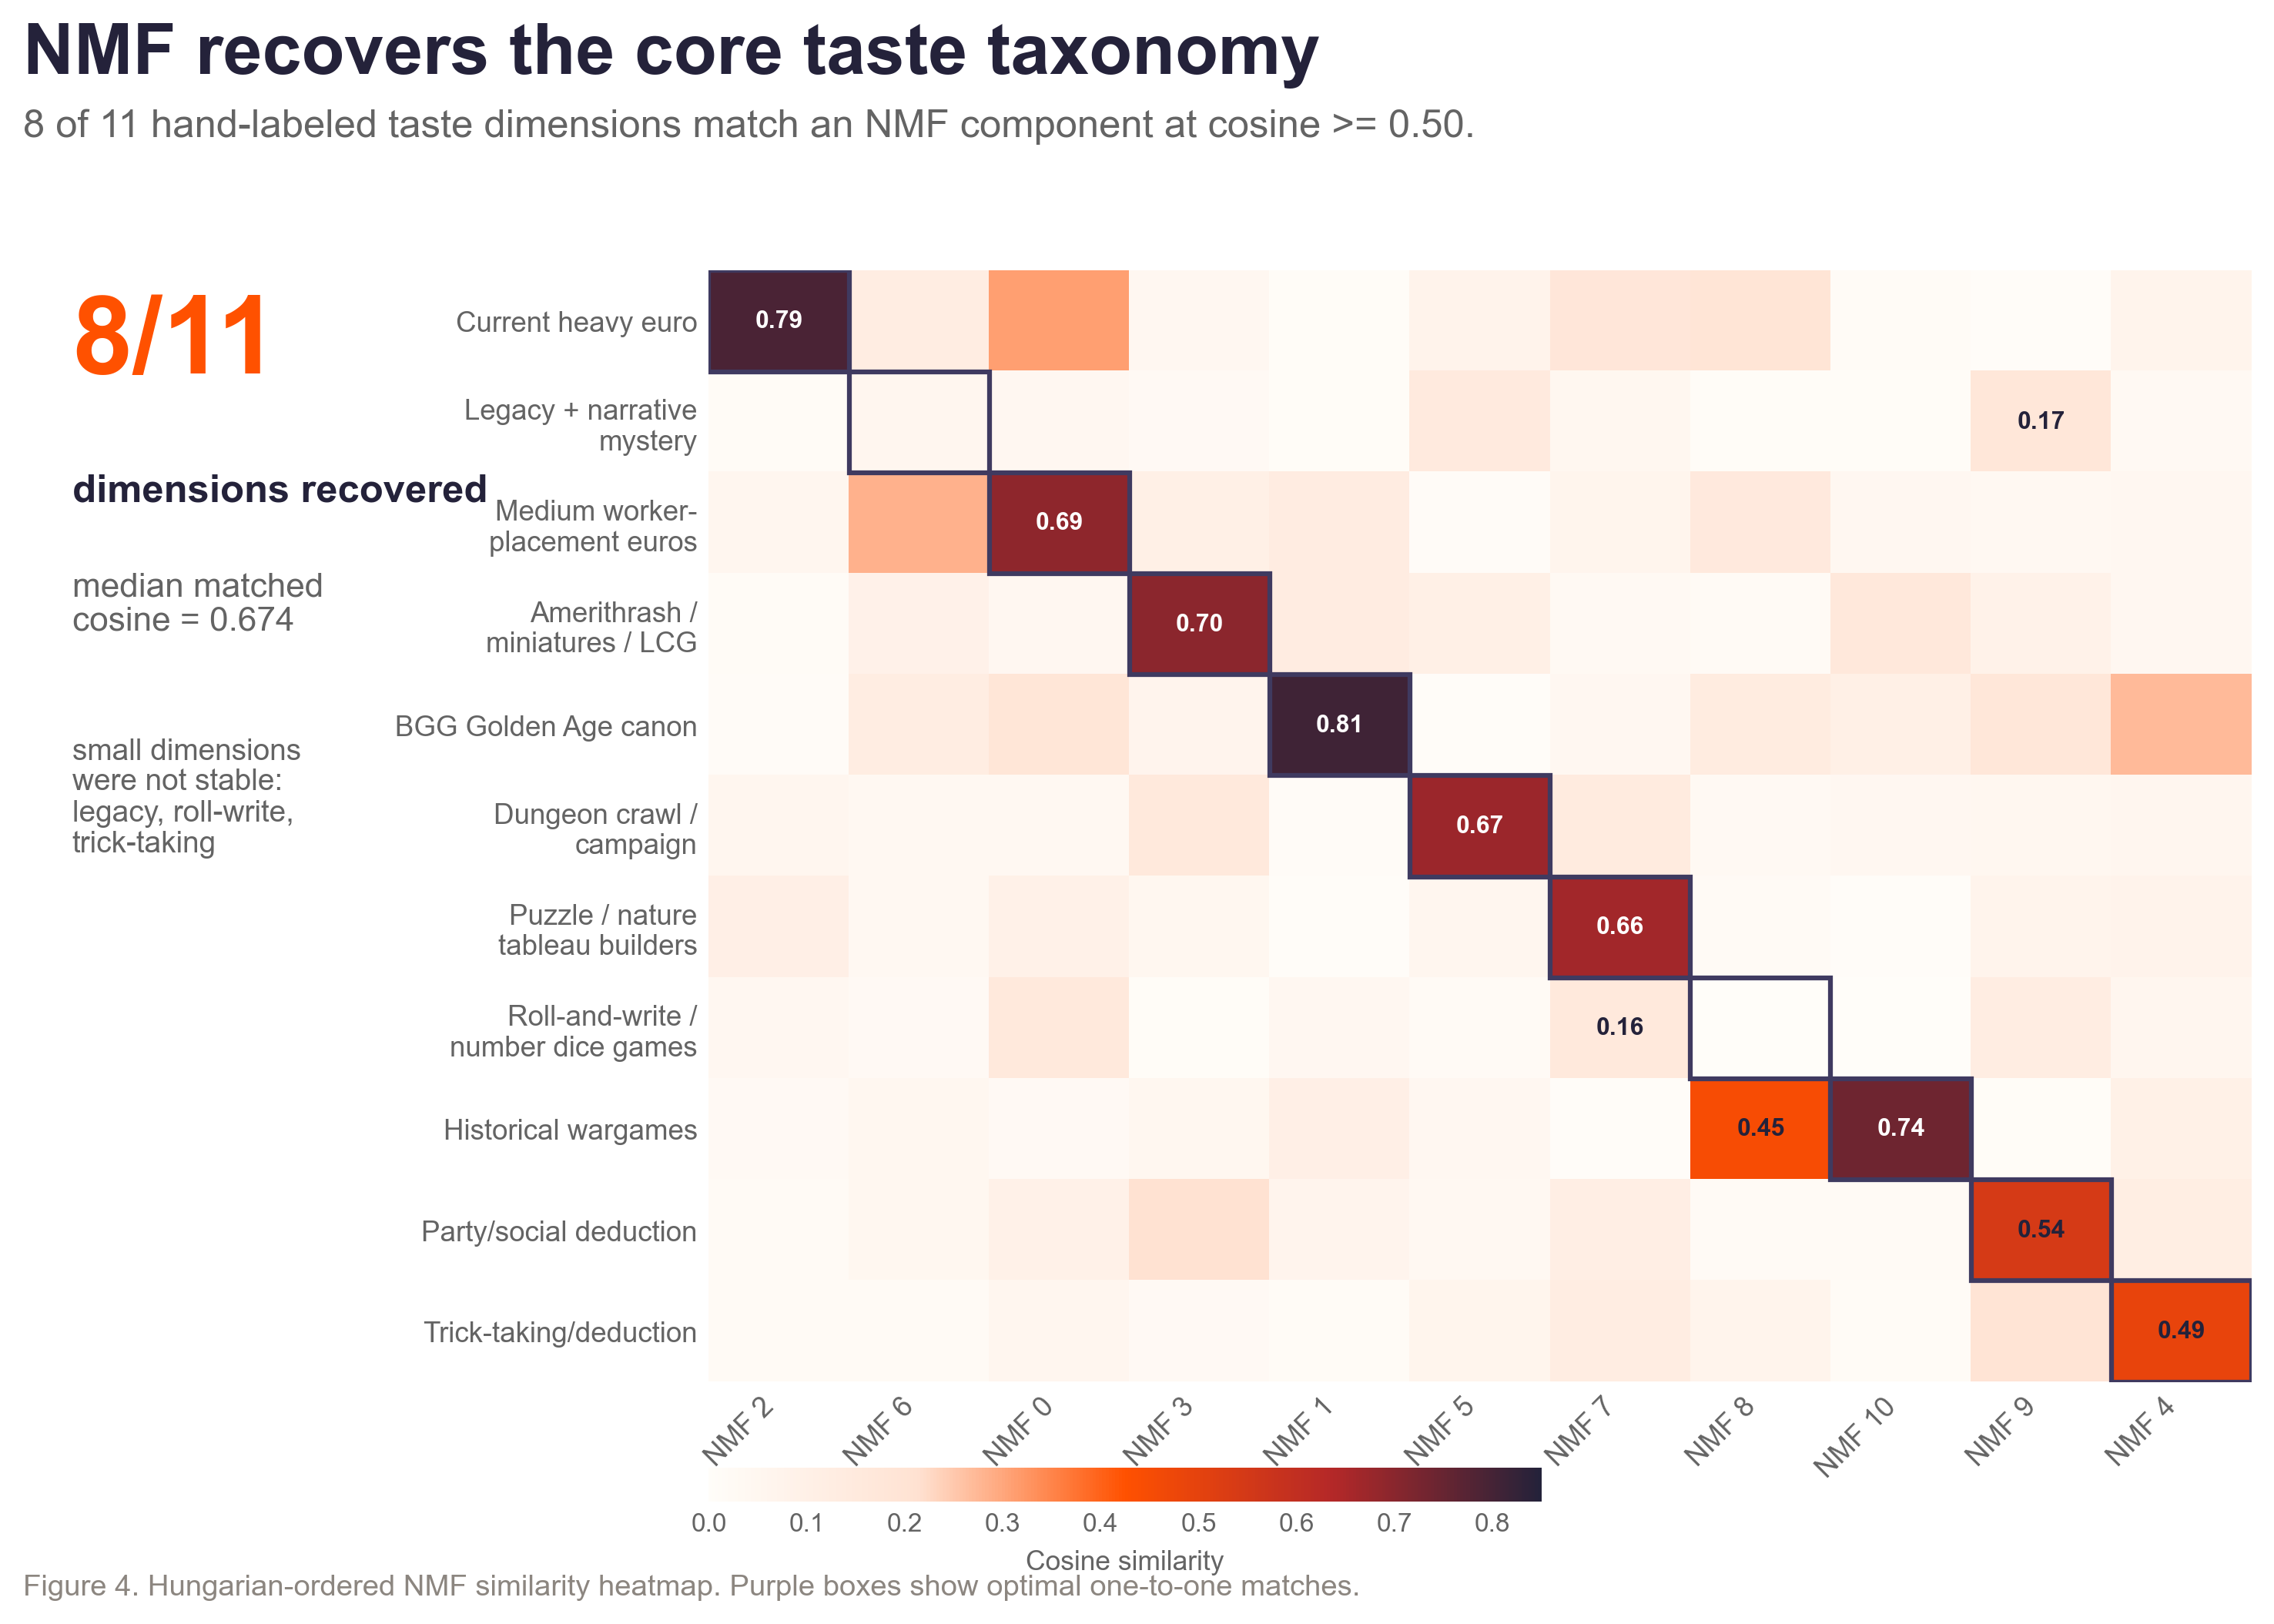
\includegraphics[width=\linewidth]{figure_nmf_validation_heatmap.png}
\caption{Cross-method validation between Louvain-derived taste dimensions and NMF components. Louvain dimensions are binary game indicators, while NMF components are continuous game-weight vectors.}
\label{fig:nmf}
\end{figure}

\section{Community Typology}

The validated midline graph produced 43 behavioral communities. Manual inspection showed that not all communities represented the same kind of structure. Some were taste identities, while others reflected hobby era, recency, franchise ownership, or bridge-game behavior.

\subsection{Structural Types}

The final typology used nine structural types, which were taste specialist, taste cross-over, temporal canon, temporal artifact, bridge cluster, bridge singleton, shared culture, franchise/series, and tiny fragment. Table \ref{tab:dims} lists the 11 dimensions used for user taste profiling.

\begin{table}[!htbp]
\centering
\footnotesize
\caption{Eleven named dimensions used for user taste profiling.}
\label{tab:dims}
\setlength{\tabcolsep}{2pt}
\begin{tabular}{@{}r p{0.45\linewidth} r p{0.25\linewidth}@{}}
\toprule
ID & Dimension & Games & Type \\
\midrule
10 & BGG Golden Age canon & 338 & temporal canon \\
9 & Amerithrash / miniatures / LCG & 251 & taste specialist \\
12 & Dungeon crawl / cooperative campaign adventure & 231 & taste specialist \\
2 & Current heavy euro engine builders & 207 & taste specialist \\
20 & Historical wargames + conflict strategy & 198 & taste specialist \\
25 & Party / family / social deduction & 177 & taste cross-over \\
13 & Puzzle / nature tableau builders & 168 & taste cross-over \\
8 & Medium worker-placement euros & 166 & taste specialist \\
35 & Cooperative trick-taking + deduction & 100 & taste cross-over \\
17 & Roll-and-write / number dice games & 39 & taste cross-over \\
4 & Legacy + narrative mystery & 37 & shared culture \\
\bottomrule
\end{tabular}
\end{table}

\begin{figure}[!htbp]
\centering
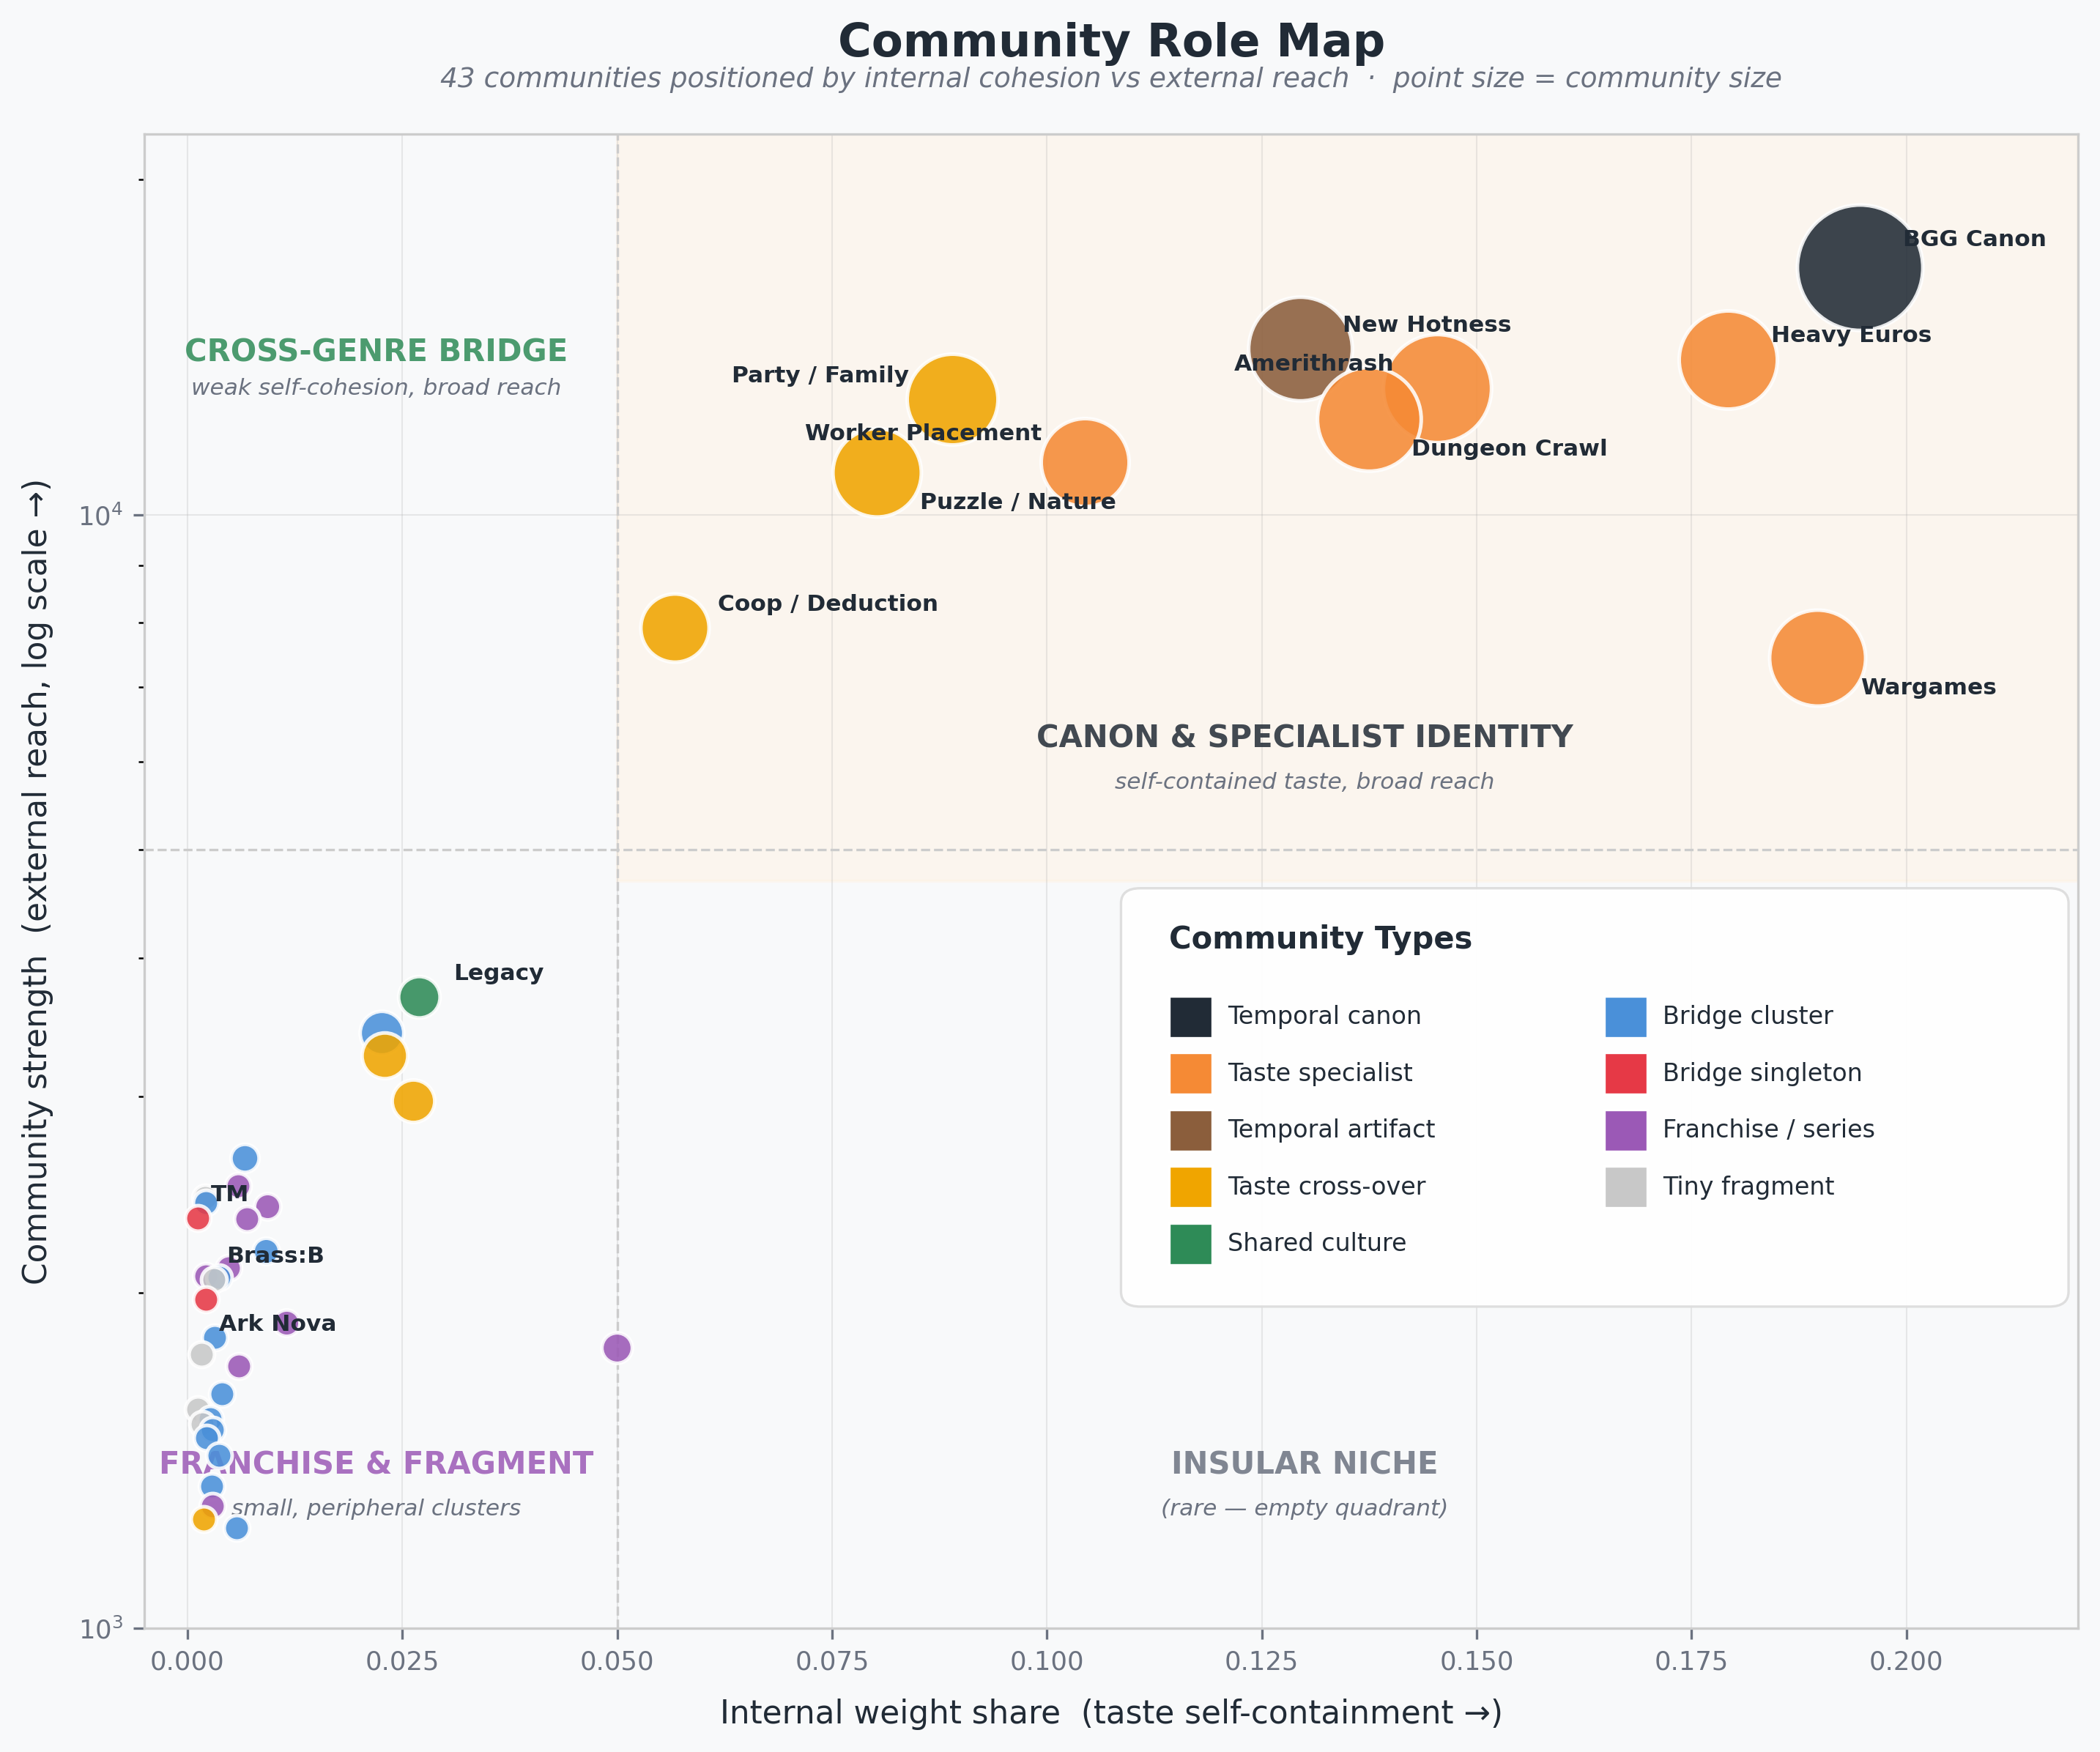
\includegraphics[width=\linewidth]{figure_role_map.png}
\caption{Community role map. Communities are placed by internal weight share, which measures taste self-containment, and by external reach.}
\label{fig:role_map}
\end{figure}

\begin{figure}[!htbp]
\centering
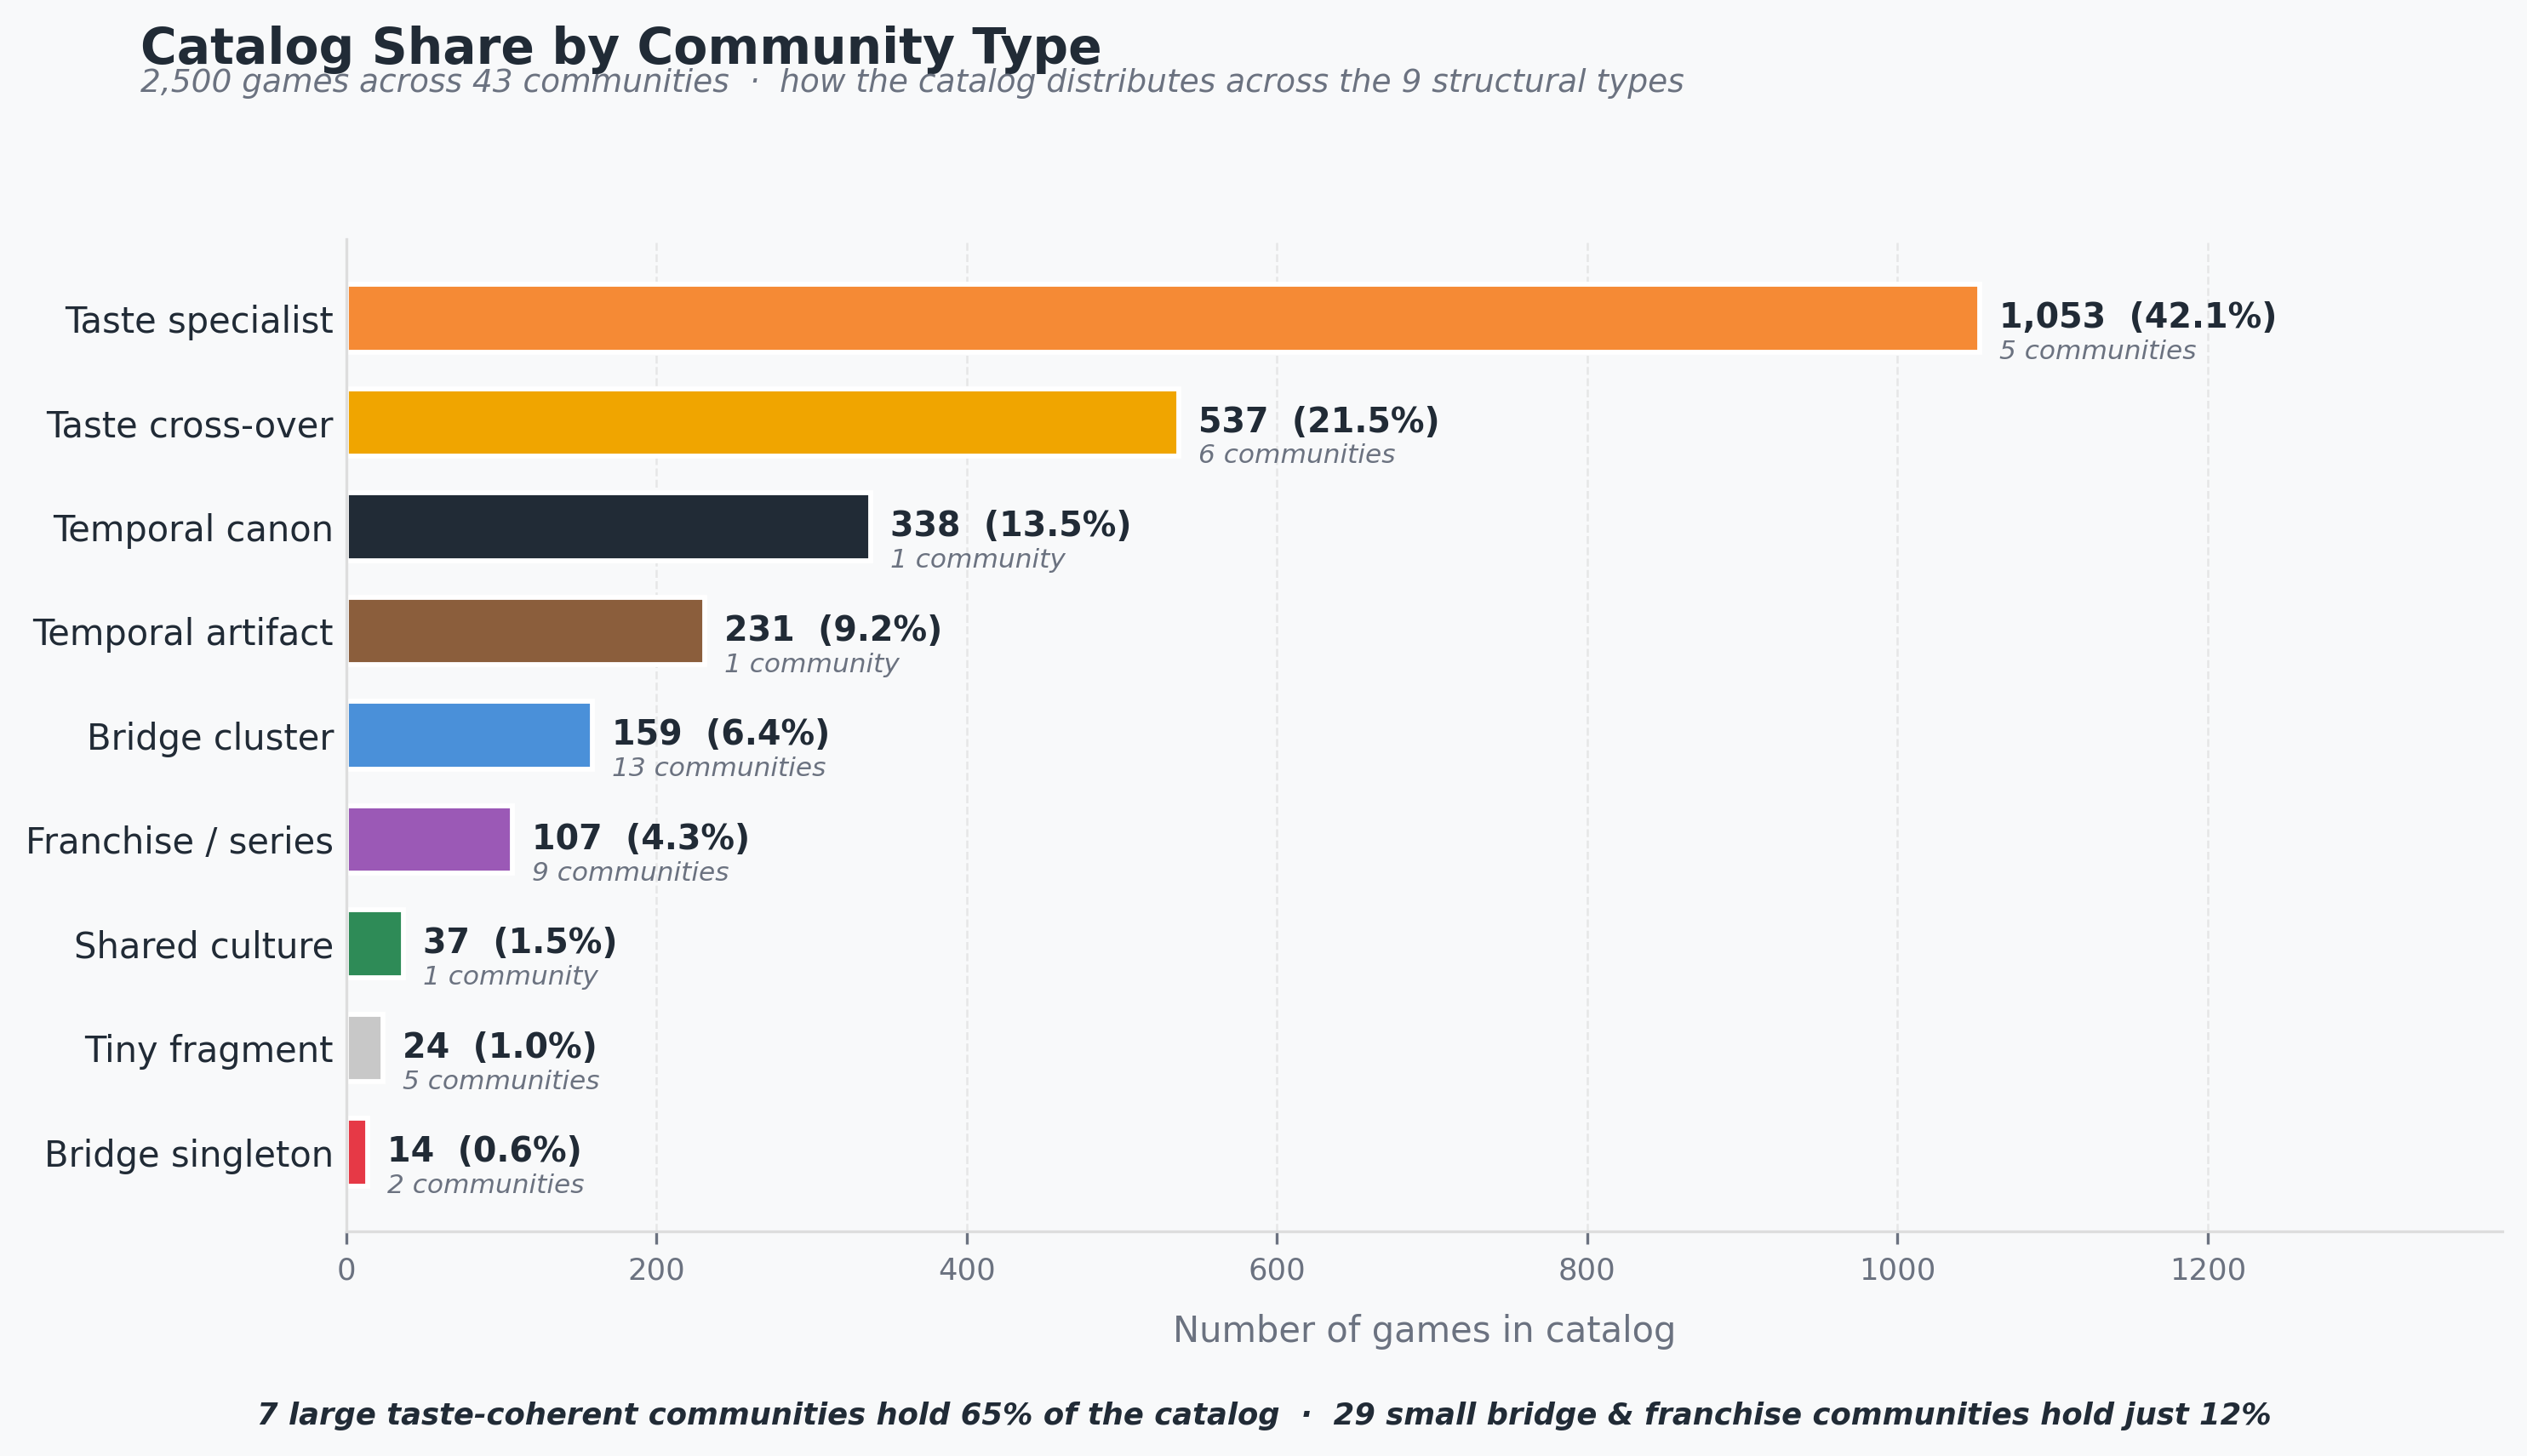
\includegraphics[width=\linewidth]{figure_catalog_share.png}
\caption{Catalog share by community type. Most games fall into taste-specialist or taste-cross-over communities, while the remaining games are distributed across temporal, bridge, franchise, shared-culture, and fragmentary structures.}
\label{fig:catalog_share}
\end{figure}

Figure \ref{fig:role_map} maps each community by structural role. For a community $c$, let $w^{\mathrm{int}}_c=\sum_{i<j,\;i,j\in c}w_{ij}$ denote internal weight and let $w^{\mathrm{ext}}_c=\sum_{i\in c,\;j\notin c}w_{ij}$ denote external weight. The internal weight share is
\begin{equation}
\frac{w^{\mathrm{int}}_c}{w^{\mathrm{int}}_c+w^{\mathrm{ext}}_c}.
\end{equation}
The role map uses this value on the horizontal axis and uses external reach, measured as $w^{\mathrm{ext}}_c$ on a log scale, on the vertical axis.

The upper-right region contains canon and specialist identities. The upper-left contains broad cross-genre bridge communities. The lower-left contains franchise fragments and small clusters. The lower-right ``insular niche'' region is nearly empty, suggesting that in this engaged BGG sample even specialized communities tend to connect outward through the shared hobby canon.

Figure \ref{fig:catalog_share} shows the catalog share of each structural type. Taste-specialist communities account for 1,053 games (42.1\%), taste-cross-over communities account for 537 games (21.5\%), and the temporal canon accounts for 338 games (13.5\%). Together, these three taste-coherent types hold about 77\% of the catalog. The remaining six structural types share about 23\% of games across many smaller communities, which is why the non-taste layer appears as a collection of bridge, franchise, temporal, and fragmentary structures rather than as one large cluster.

\subsection{Main Community Findings}

Historical wargames formed one of the cleanest specialist identities, with deep niche ownership and strong internal self-containment. Metadata enrichment supports this interpretation. Community 20 showed 7.20$\times$ enrichment for the Wargame category, 8.44$\times$ for the Simulation mechanic, and 11.84$\times$ for Ratio / Combat Results Table.

The BGG Golden Age canon captured older hobby-defining games such as \emph{Puerto Rico}, \emph{Agricola}, \emph{Power Grid}, \emph{Ra}, and \emph{Tigris \& Euphrates}. Modern heavy euros, dungeon-crawl campaigns, and Amerithrash/LCG games appeared as separate specialist identities. By contrast, party games, puzzle/nature games, trick-taking, and legacy games behaved more like supplementary or cross-over layers.

\subsection{Bridge Singletons}

Several highly ranked games did not anchor a single taste community. \emph{Brass: Birmingham} (BGG rank \#1), \emph{Ark Nova} (\#2), and \emph{Terraforming Mars} (\#9) appeared as bridge singletons or universal-appeal micro-clusters rather than as clean members of one specialist group. This is not a popularity statement alone. The structural interpretation is that extreme broad appeal reduces community specificity because these games are owned by many kinds of collectors. They therefore function more as shared cultural objects than as markers of one taste identity.

\subsection{Temporal Artifact}

The recent-release community grouped games such as \emph{Sky Team}, \emph{SCOUT}, \emph{Heat}, \emph{Harmonies}, and \emph{Dune: Imperium -- Uprising}. These games are not unified by one mechanic or theme. They are unified by time. Co-ownership therefore captures the BGG new-hotness cycle, a temporal behavior that metadata categories alone cannot represent.

\section{User Taste Profiling}

After community labeling, each eligible user was represented as a 12-dimensional profile made of 11 named dimensions plus one residual ``other'' bucket. The residual bucket pooled the remaining 32 communities, including temporal artifacts, bridge clusters, franchise clusters, bridge singletons, and tiny fragments. Users were eligible for archetype classification if they owned at least 15 selected games. This threshold was used because profiles below 15 selected games are too sparse for a stable 12-dimensional characterization.

The classification rules were explicit.

\begin{itemize}
    \item Other-dominant means that the largest profile dimension is the residual ``other'' bucket.
    \item Specialist means that the dominant named taste share is at least 0.40.
    \item Generalist means that normalized entropy is at least 0.75 and dominant share is below 0.35.
    \item Leaning means that dominant named taste share is at least 0.25 after failing the specialist and generalist gates.
    \item Mixed contains the remaining eligible cases.
\end{itemize}

Profile entropy was normalized by the logarithm of the number of dimensions so that 0 means a narrow profile and 1 means a maximally even profile. Figure \ref{fig:user_insight} summarizes the resulting user-side pattern.

\begin{figure}[!htbp]
\centering
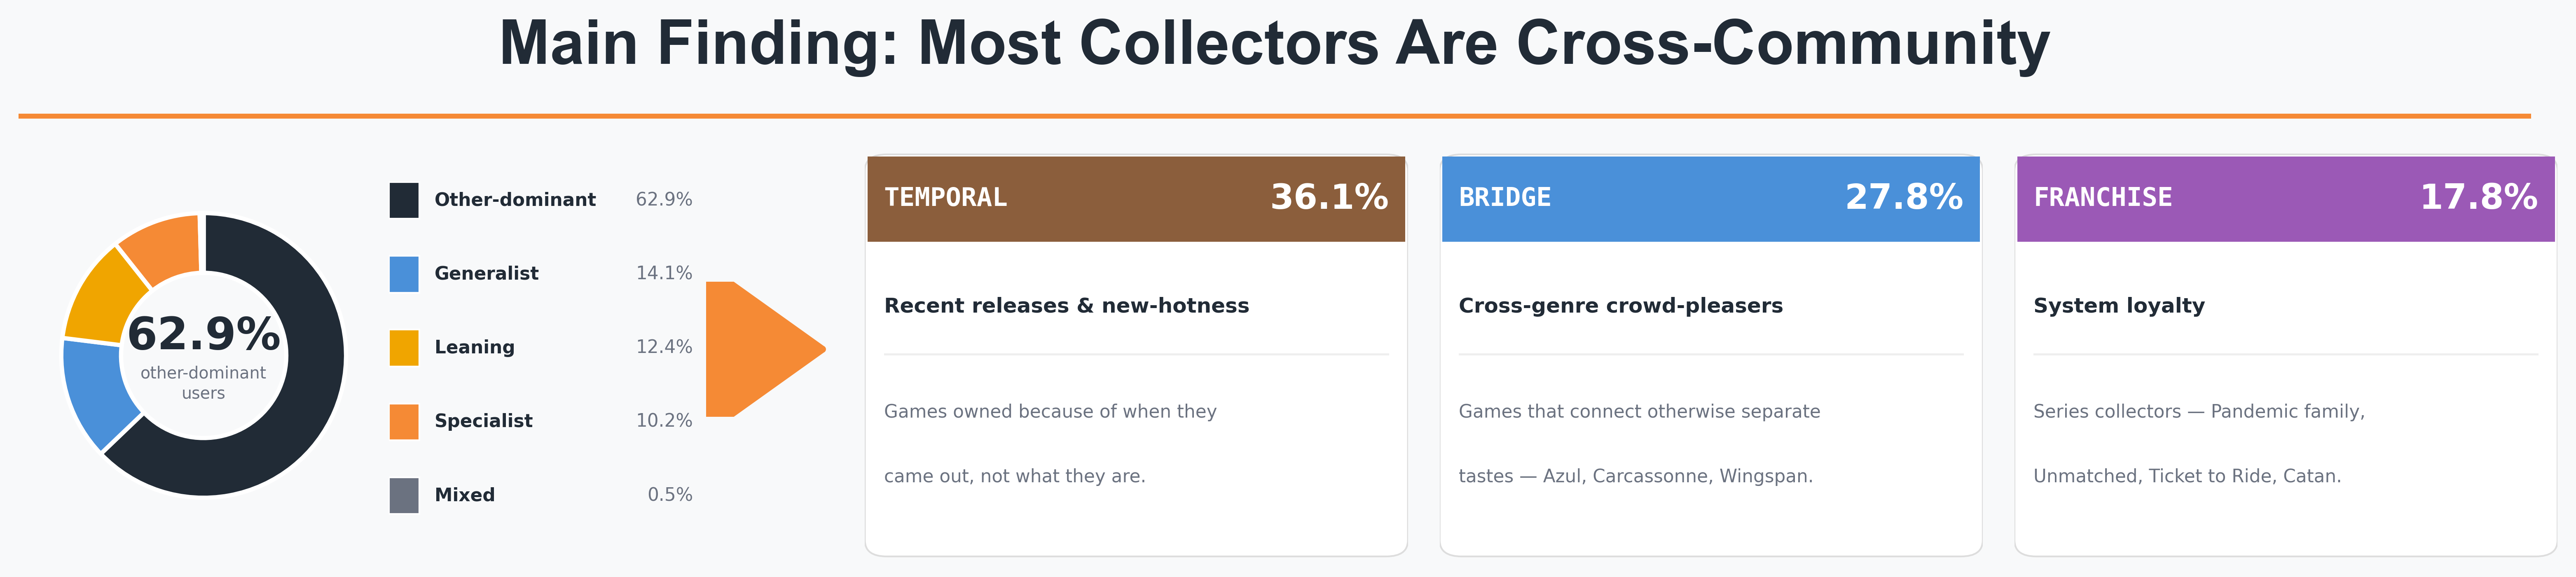
\includegraphics[width=\linewidth]{figure_main_finding_hero.png}
\caption{Main user insight. Most eligible users are not dominated by one named taste community. Their residual ownership decomposes into temporal, bridge, and franchise modes, suggesting a shared-canon layer that cuts across taste identities.}
\label{fig:user_insight}
\end{figure}

\begin{table}[!htbp]
\centering
\caption{Eligible user archetype distribution.}
\label{tab:users}
\begin{tabular}{lrr}
\toprule
Archetype & Users & Eligible share \\
\midrule
Other-dominant & 3,221 & 62.9\% \\
Generalist & 723 & 14.1\% \\
Leaning & 634 & 12.4\% \\
Specialist & 524 & 10.2\% \\
Mixed & 23 & 0.4\% \\
\bottomrule
\end{tabular}
\end{table}

\begin{table}[!htbp]
\centering
\caption{Decomposition of ownership edges inside the other-dominant residual layer.}
\label{tab:other}
\begin{tabular}{lr}
\toprule
Residual source & Share \\
\midrule
Temporal artifact & 36.1\% \\
Bridge cluster & 27.8\% \\
Franchise/series & 17.8\% \\
Taste cross-over & 7.9\% \\
Tiny fragment & 7.2\% \\
Bridge singleton & 3.2\% \\
\bottomrule
\end{tabular}
\end{table}

The main user-level result is that 62.9\% of eligible collectors are other-dominant. This does not mean that the profiling failed. The residual bucket decomposes into meaningful non-taste structures, mainly temporal artifacts, bridge clusters, and franchise systems. The user-side pattern mirrors the game-side bridge singleton finding because many collectors and many highly ranked games are organized by a shared-canon layer rather than by one stable genre identity.
The mixed family contains only 23 users, or 0.4\% of eligible users, so it should be interpreted as a small residual from the threshold rules rather than as a substantive collector type.

\section{Validation and Metadata Alignment}

The project used several validation layers. First, the selected Louvain partition was stable across 20 random seeds, with median pairwise NMI $=0.758$. Second, the observed modularity exceeded the degree-preserving null model with $z=27.31$. Third, NMF recovered 8 of 11 Louvain-derived dimensions directly from the raw ownership matrix. Fourth, metadata was used as an external validation source after community detection.

Metadata alignment was moderate rather than overwhelming. Behavioral backbone edges had mean mechanics Jaccard 0.091 versus 0.065 for random game pairs, and mean category Jaccard 0.098 versus 0.058 for random game pairs. In simpler terms, behavioral edges shared at least one mechanic 64.3\% of the time, compared with 49.0\% for random game pairs, and they shared at least one category 38.0\% of the time, compared with 24.5\% for random pairs. This corresponds to roughly 1.39$\times$ lift for mechanics Jaccard and 1.70$\times$ lift for category Jaccard.

This result is important because it positions metadata correctly. Mechanics and categories partially explain co-ownership, but they do not exhaust it. The gap between metadata similarity and behavioral structure is where temporal artifacts, bridge games, franchise systems, and shared-canon behavior become visible.

\section{Limitations and Future Work}

The dataset is not a random sample of all BGG users. It is a dense engaged-user dataset with targeted expansion toward underrepresented tags. This makes it appropriate for studying active collector behavior, but not for estimating the behavior of casual or inactive BGG accounts.

The projection step also simplifies the original bipartite structure. Newman normalization reduces heavy-collector dominance, but any game-game projection discards some user-level information. NMF partially addresses this by operating directly on the raw matrix, but future work could apply bipartite-native community detection, Leiden robustness checks, or predictive recommendation tests.

Temporal information is also only indirectly used. The recent-release community suggests that time strongly shapes co-ownership, but the present analysis does not model collection growth or acquisition dates. A future temporal network or tensor decomposition could separate stable taste identity from release-cycle dynamics more directly.

Finally, the user profile categories depend on manual grouping of communities into dimensions and on threshold choices for archetype classification. These categories are useful summaries, but they should not be interpreted as fixed psychological labels.

\section{Conclusion}

BGG ownership behavior is structured, but not only by genre or metadata. The network analysis reveals coherent taste communities, including wargames, heavy euros, dungeon-crawl campaigns, Amerithrash/LCG games, party/social games, and medium worker-placement euros. Matrix decomposition independently recovers most of the same taste dimensions, supporting the data-driven nature of the taxonomy.

The strongest result is the shared-canon layer. A majority of eligible collectors are not dominated by one taste identity. Instead, their collections are organized by temporal trends, bridge games, and franchise systems. The same pattern appears on the game side: some of the most broadly owned games do not anchor one community because they function as shared cultural objects across communities.

The final answer to the research question is therefore two-layered. BGG ownership contains differentiated taste identities, but it also contains a shared canon that cuts across them. Co-ownership exposes the boundary between taste identity and shared culture in a way that ratings, rankings, or metadata alone cannot. The methodological contribution is the dual-method screening protocol, where graph-side community detection and matrix-side decomposition validate and refine each other. This approach can be transferred to other co-ownership and co-engagement networks.

\balance

\section*{Acknowledgments}

This project was completed for CS514 Network Science at Sabanc\i{} University. Course discussions and project feedback helped shape the methodological choices and final framing. BoardGameGeek data and public API access made the analysis possible.

\begin{thebibliography}{9}

\bibitem{newman2001}
M. E. J. Newman.
\newblock Scientific collaboration networks. II. Shortest paths, weighted networks, and centrality.
\newblock \emph{Physical Review E}, 64(1):016132, 2001.

\bibitem{serrano2009}
M. A. Serrano, M. Boguna, and A. Vespignani.
\newblock Extracting the multiscale backbone of complex weighted networks.
\newblock \emph{Proceedings of the National Academy of Sciences}, 106(16):6483--6488, 2009.

\bibitem{blondel2008}
V. D. Blondel, J.-L. Guillaume, R. Lambiotte, and E. Lefebvre.
\newblock Fast unfolding of communities in large networks.
\newblock \emph{Journal of Statistical Mechanics: Theory and Experiment}, 2008(10):P10008, 2008.

\bibitem{lee2001}
D. D. Lee and H. S. Seung.
\newblock Algorithms for non-negative matrix factorization.
\newblock \emph{Advances in Neural Information Processing Systems}, 13, 2001.

\bibitem{traag2019}
V. A. Traag, L. Waltman, and N. J. van Eck.
\newblock From Louvain to Leiden: guaranteeing well-connected communities.
\newblock \emph{Scientific Reports}, 9:5233, 2019.

\bibitem{bgg}
BoardGameGeek.
\newblock Board game rankings, metadata, and user collection records.
\newblock \url{https://boardgamegeek.com/}.

\end{thebibliography}

\end{document}
